\chapter{引言}
\section{研究背景}
% 介绍图计算

%图计算很有用
图(Graph)是一种重要的数据结构,它由节点 V(或称为顶点,即个体),与边 E(即个体之间的联系)构成。
图能够对很多问题进行抽象建模。
比如在facebook、twitter、weibo这些社交网络中,我们可以把用户看作顶点,
把用户之间建立的关系看作边,这样就能用图来研究社交网络中的各种规律。
在互联网中通过把web网页看作顶点,
把页面之间的超链接看作边,就可以通过图来研究网页的权重排名信息。
而随着大数据时代的到来,如何对海量图数据进行高效的处理分析愈加成为工业和学术界的研究热点。

\begin{figure}[!htbp]
  \centering
  
\includegraphics[width=0.40\textwidth]{graphs_are_everywhere.png}
  \bicaption{图计算的重要性}{The importance of graph computing}
\end{figure}

%人们开发了很多框架进行图计算
传统的大数据处理平台使用MapReduce\cite{mapreduce}这种函数式编程范式,但这种编程范式并不适用于图计算。
基于函数式编程思想的MapReduce需要在每次迭代之间传递数据,
而图计算由于结构内在的复杂性,计算往往是不规则的,计算过程中很多数据不需要传递。
并且图算法若要用MapReduce实现往往需要转换为一系列MapReduce任务,这又会带来额外的存储读写开销,
所以传统的大数据处理平台无法胜任大规模图计算任务\cite{Malewicz@SIGMOD10}。
为此人们开发了许多专门用于处理大规模图数据的分布式并行计算框架。    
\cite{Malewicz@SIGMOD10, Low@12, Gonzalez@OSDI12, Zhu@OSDI16, Gonzalez@OSDI14, Avery@HS11, Shao@SIGMOD13, 
Chen@EuroSys15, Xie@PPoPP15, Roy@SOSP15, Seo@CloudCom10, Gregor@POOSC15, Hoque@TRIOS13, Teixeira@SOSP15}

\section{针对副本点的延迟数据一致性方法}

%介绍副本点
由于大规模图数据要在集群中分布式存储, 因此副本点在现有的分布式图计算编程框架中充当着关键角色。
% 这些图计算框架都要把大规模图数据在集群中分布式存储,因此副本点在现有的分布式图计算编程框架中充当着关键角色。  
副本点使得集群中的多台机器可以对一个顶点$v$并行地计算,同时也使得每个顶点可以在本地访问远程顶点,减少了机器之间的通讯开销。 
图\ref{fig:mirror}展示了一个小图在4台机器上划分后的结果,可以看到中心的顶点产生了4个副本点。

\begin{figure}[!htbp]
  \centering
  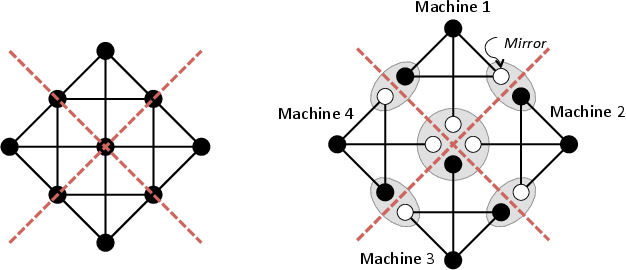
\includegraphics[width=0.40\textwidth]{mirror}
  \bicaption{副本点示意图}{schematic diagram of mirror vertex}
  \label{fig:mirror}
\end{figure}

%副本点存在的问题
然而副本点在带来巨大好处的同时也引入了数据一致性的问题。
分布式图计算编程框架要维护不同机器上存储的副本点$v_1, v_2, \cdots, v_k$之间的数据一致性。
很多编程框架都把每个顶点看做一个原子性的点,使用 eager data coherence 的方法来保证所有副本之间的数据是一致的,
每个点横跨的机器数量和数据同步频率直接影响系统通信量的大小进而影响系统的性能。
在这种方法中,系统把顶点$v$的副本点中的其中一个标记为master点,其他副本点为mirror点,其中master点保存了该顶点的真实数据,
而mirror点只实时地保存着master点数据的一份本地拷贝。
对顶点$v$的所有更新必须在master点上进行,更新完成后都会立即通过消息传递把最新状态发送给所有副本,这带来了频繁的全局同步和消息通信。

%lazygraph 的解决思路
针对这一问题,我们提出了一种延迟数据一致性方法(lazy data coherence,LazyAsync)\cite{Wang@PPoPP18}有效地降低了系统用于维护副本点数据一致性的开销。
我们发现,通过把算法每次迭代的公式改写为差值累加的形式,各副本点通过交换差值消息即可达到数据一致,
这样就消除了顶点计算过程中产生的数据同步和消息交换。
此外对于绝大多数图算法,系统时刻维护副本点之间的数据一致性并不是必须的。
对于一些经典的图算法某个点的解往往只依赖于它部分的邻居节点,而对于数据挖掘和机器学习类的图算法中间过程的不一致往往不会影响最终的收敛性。
我们进一步通过数学公式推演证明迭代公式改写为差值累加的形式之后,
各副本点可以各自独立地进行数轮本地计算后再进行差值消息交换实现数据一致,
而不必在每次迭代之后就进行差值消息交换,它们最终得到的结果是等价的,
这样我们就可以进一步减少系统中进行数据同步和全局消息交换的开销。

%lazygraph 的效果
由于单个迭代计算过程中副本点之间不必同步,多轮迭代计算过程之间副本点之间可以延迟同步,
系统极大地减少了全局数据同步和通信的开销。
基于这些发现,我们把副本点看做是互相独立的迭代更新自己的数据的顶点,
% 各自进行数次迭代计算之后通过交换差值累加消息实现副本点之间的数据一致性
  各自进行数次迭代计算之后通过在同样的差值累加消息上进行计算来实现副本点之间的数据一致性,
并最终在具有代表性的分布式并行图计算框架PowerGraph\cite{Gonzalez@OSDI12}上实现了这种延迟数据一致性方法。
在48个虚拟机的EC2的集群环境下的实验结果表明,在4种典型的图算法和不同种类的真实输入图上,我们这种方法在保证正确性的基础上,
相较于PowerGraph获得了1.25倍到10.69倍的加速比。


\section{延迟数据一致性方法尚未解决的问题}
% lazygraph 的性能提升效果依赖于具体的延迟一致开启策略
% lazygraph 现在采用一个决策树模型作为开启策略,它存在着以下这些方面的不足
% 1. 难以解释
% 2. 训练过程依赖于手动调优
% 3. 无法做到自适应
虽然我们提出的延迟数据一致性方法极大的提升了分布式图计算的性能,但是它在以下这几个方面还存在着一系列尚未解决的问题。    
\begin{enumerate}      
  \item[(一)] 延迟同步策略和系统得到性能提升相对大小之间的关系有待研究 \newline\indent
    何时开启延迟同步?延迟同步开启多久进行数据一致?
    随着这些具体策略的不同,系统得到的加速比也不同。
    要想得到相对最优的效果,研究清楚延迟同步如何影响性能提升是有必要的。

  \item[(二)] 目前系统实现的决策树方法存在缺陷 \newline\indent
    延迟数据一致性方法需要结合具体的应用算法和输入图选择合适的时间节点进行数据一致。
    目前的系统实现中采用的是通过离线训练得到的决策树模型,这种模型需要对算法和输入图组合手动调优,耗费时间较长,
    并且对于新的算法和输入图组合不能保证得到相对最优的性能提升,这对于一个实用的图计算系统来说是不可接受的。
    因此我们需要对目前的系统实现进行改进,把这个过程自动化,使得系统的模型具有足够的泛化能力,能够自适应的处理各种输入。          

  \item[(三)] 目前的系统缺乏一个考虑各种影响因素的自适应优化策略 \newline\indent
    %how to say?
    虽然我们提出了一种行之有效证明正确的延迟一致性方法,但是这个方法目前还缺乏一个自适应各种影响因素的优化策略。
    对于采用了延迟数据一致性的分布式并行图计算系统,除了延迟一致性开启策略之外,具体的算法用例,
    输入图结构特征,图划分算法,配置环境等都会对最终的性能造成影响,并且在系统执行过程中这些因素是动态变化而又互相影响的,
    为了得到相对最优的性能提升效率,系统需要一个能够自适应这些外部因素的优化策略,实时监控这些因素动态地调节全局同步的频率。          
    % 以及目前的系统实现中只在同步引擎上实现了延迟一致性方法,而有些算法更适合异步引擎,因此这种方法是否能够应用到异步引擎中也有待研究。
\end{enumerate}
\section{基于解的局部性的自适应优化方法}
% 通过实验发现, 解存在着局部性规律可以作为自适应开启策略
为了解决延迟数据一致性方法目前存在的问题,本文首先对这种方法的性能提升规律进行了研究。
在之前的工作中,我们从分布式计算系统的角度解释了延迟一致性方法的性能收益的来源。
延迟一致性方法减少了图计算的迭代次数,极大的降低了系统的全局同步等待和集群之间的通信这些开销,
从而得到了性能提升。
但是这种阐述只能说明延迟一致性方法方法能够提升性能这个定性的问题,
却无法回答延迟一致性方法在不同的开启策略下得到不同程度的性能收益这种定量的问题。
而且在实际的实验中我们发现,在某些情况下延迟一致方法虽然减少了迭代次数,但是最终却并没有拿到计算时间上的性能收益。

通过定义有效计算的概念,我们最终发现了延迟一致性方法的性能提升的相对大小的规律。
我们发现延迟数据一致性方法虽然避免了急切数据一致性方法中存在的冗余的同步,等待和通信,
但是却有可能在本地计算中引入新的冗余计算。
在延迟一致性方法不同的开启策略中,那些性能提升更好的情况是因为进行了更多的有效计算,
而那些性能提升相对不好的情况则是因为进行了更多的冗余计算。
所以,延迟一致方法要想得到相对最优的性能提升,就要从提高有效计算的比例入手。

通过分析,我们发现延迟一致方法能否进行更多的有效计算和顶点上的全局解和局部解的关系规律有关。
在分布式图计算中,由于副本点的存在,每个顶点上的全局解由多个局部解构成。
延迟一致性方法通过在数据一致性节点通过交换构成局部解的消息累加值来实现不同副本点上的全局解的一致。
而在数据一致性节点之间,各个副本点上在本地进行不需要消息交换和通信的本地计算。
这些本地计算能维持较高的有效计算的比例时,延迟一致性方法就能获得较高的性能收益。

另一方面,当顶点上的全局解只由一个局部解构成时,本地计算就能进行更多的有效计算,
当顶点上的全局解由多个局部解构成时,本地计算就容易造成更多的无效计算。
也就是说,当活跃点中的大多数点的全局解都只由单个局部解构成,
或者全局解由多个局部解构成的点的数量在下降时,
延迟一致性方法就能够通过多轮的本地计算对本地子图进行事先的有效计算,
最终得到较好的性能收益。


全局解和局部解的关系影响着延迟数据一致性方法的有效计算的程度,进而影响了这种方法的性能提升相对大小。
经过一系列实验之后,我们进一步找到了全局解和局部解的关系变化规律。
我们发现,在图计算过程中,随着计算的进行,全局解由多个局部解构成的点的数量会逐渐下降,
并且在每轮的活跃点中只占一小部分比例。
也就是说,随着计算的进行,图计算中的点的全局解大部分是由单个局部解所决定构成的,
我们可以称之为解的局部性。
正是由于解的局部性的存在,延迟数据一致性方法才能通过延迟同步本地计算来减少系统中数据交换从而获得性能收益。

然而解的局部性并不是一直存在的,这也是延迟数据一致性方法需要合适的开启策略的原因。
通过实验我们发现,解的局部性和具体的输入图和算法用例以及集群的配置有关。
随着这些外部输入条件的不同,解的局部性也有着不同的变化规律。
在有的组合中,一开始就一直呈现出较为明显的解的局部性的规律,即全局解由多个局部解构成的顶点一直只占极少一部分。
而在有的组合中,一开始解的局部性现象并不存在,而是存在着全局解由多个局部解构成的顶点数量一直在增长的过程。
当这样的顶点数量在增长时,是不适宜开启延迟数据一致性方法的。

在之前的工作中,我们通过机器学习的手段找到了一个决策树模型作为开启策略。
这个决策树使用输入图的边点比例和运行时的活跃点变化趋势作为开启策略的判断条件。
通过实验我们发现,决策树所使用的特征其实也是对解的局部性变化规律的间接反映。
% 同时,由于决策树是对手动调优产生的训练集的数据拟合

最终,通过在运行时动态的监控全局解由多个局部解构成的顶点的数量和比例,我们得到了一个基于解的局部性的自适应优化方法。
这个自适应优化方法在动态观察到图计算迭代过程中开始存在解的局部性时,就开启延迟数据一致性方法。
这种方法克服了之前的决策树模型存在的失灵问题,同时也不需要事先的手动调优产生数据集来进行训练。
此外,由于解的局部性是受输入图特性,算法用例,集群配置环境所共同影响的,所以这种方法能够实现对这些不同外部输入条件的自适应。

总而言之,本文的主要创新点和贡献可以归纳为以下几点:

1. 对延迟数据一致性方法的在不同开启策略下得到不同性能提升这一现象进行了研究,认清了这一方法的性能提升规律。
以具体的例子识别出了延迟数据一致性方法虽然避免了急切数据一致性方法存在的冗余同步和通信,但是引入了新的冗余计算。
并且正是这种冗余计算造成了延迟数据一致性方法在不同开启策略性下得到不同程度的性能提升。

2. 对图计算过程中活跃点上全局解和局部解之间的关系进行了研究,发现了解的局部性这一现象。
通过分析,本课题发现随着图计算的进行,每次迭代中大部分活跃点的全局解只由某个局部解构成,
那么此时局部解所在的副本点完全不需要等待和同步其他副本点就可以继续进行图计算过程。
而这种情况正是有利于减少冗余计算,有利于开启延迟数据一致性方法的情况。

3. 基于解的局部性这一现象,实现了基于解的局部性的自适应优化方法。
这种方法解决了延迟数据一致性方法在不同的输入条件下如何得到相对最优的性能提升这一问题。
相较于之前采用的决策树方法,这种方法不需要事先的离线调优和训练,更不存在某些输入条件下失灵的问题。


%从 到 最终 我们发现了。。。


\section{全文结构}
% 每一章写了什么
本文各章节的具体内容安排如下:

第一章是引言。介绍了我们之前针对分布式并行图计算框架中副本点存在的问题所提出的延迟数据一致方法这一研究背景。
然后介绍了这个方法所遗留的问题,以及本课题针对这些问题所做的工作。

第二章是相关技术介绍及研究动机。介绍了分布式图计算中主要的研究主题,并对本课题的研究基础-延迟数据一致性方法做了重点介绍。
随后介绍了延迟数据一致性的开启策略问题,也正是本文的研究动机。

第三章LazyGraph性能提升规律研究。
首先对延迟数据一致性方法的性能收益的来源进行了研究。
从具体算法的角度,本课题展示了这种方法的性能收益来自于 它能够在本地计算所进行的额外多轮迭代中提前激活顶点并使之收敛。
然后通过分析具体的例子,本课题提出在这种本地计算中存在着冗余无效的计算,并且这些冗余计算会造成性能损失。
最后本课题通过具体的实验验证了这一观点。
从延迟一致带来的性能收益,到冗余计算带来的性能损失,本课题在这一章发现LazyGraph不同开启策略下得到不同程度的性能提升这一现象
背后的原因
正是因为本地计算中存在着相应的不同程度的冗余计算。

第四章基于解的局部性的自适应优化方法。
冗余计算影响影响收益,
本章先是介绍了全局解和局部解的关系如何影响冗余计算。
然后通过离线分析的方法,本章对不同算法和输入图上全局解和局部解之间的关系进行了实验分析,
发现了全局解和局部解之间存在着局部性关系。
接下来通过在线统计的方法,本章提出了基于解的局部性的自适应优化方法用于指导延迟数据一致性的开启策略。
最后,本章在不同算法和输入图上进行了实验评测,并对评测结果进行了分析。

最后一章对全文的研究内容进行了总结和展望。




